\documentclass[border=3pt,tikz]{standalone}
% Shared look for every TikZ figure in these notes.
% Included by each standalone figure file; also keeps the figures consistent
% with the colours used in the PDF and on the website.

\usepackage{tikz}
\usepackage{pgfplots}
\pgfplotsset{compat=1.18}
\usetikzlibrary{arrows.meta, decorations.markings, decorations.pathmorphing,
                patterns, calc, positioning}
\usepackage{amsmath}

% Series colours are the three validated categorical slots also used by the
% interactive widgets, so a path drawn in the printed notes and the same path on
% the website are the same colour. They clear the colour-vision-deficiency and
% contrast checks as a set; every path is direct-labelled as well, so colour is
% never the only thing carrying identity.
\definecolor{duPurple}{HTML}{68246D}
\definecolor{duBlue}{HTML}{2A78D6}
\definecolor{duRed}{HTML}{EB6834}
\definecolor{duGreen}{HTML}{1BAF7A}
\definecolor{duGrey}{HTML}{4D4D4D}

\tikzset{
  % heavier default lines and arrow tips, so diagrams stay clear when zoomed
  every picture/.append style = {line width=0.7pt, >={Stealth[length=3mm]}},
  axisline/.style   = {-{Stealth[length=3.4mm]}, line width=1.0pt, black},
  path1/.style      = {duBlue,   line width=1.6pt},
  path2/.style      = {duRed,    line width=1.6pt},
  path3/.style      = {duGreen,  line width=1.6pt},
  statedot/.style   = {circle, fill=black, inner sep=1.8pt},
  arrowhead/.style  = {decoration={markings,
                        mark=at position #1 with {\arrow{Stealth[length=3.4mm]}}},
                       postaction={decorate}},
  lbl/.style        = {font=\normalsize},
  slbl/.style       = {font=\small, duGrey},
  workfill/.style   = {duPurple, opacity=0.16},
}

% larger labels in plots as well
\pgfplotsset{every axis/.append style={label style={font=\normalsize}, tick label style={font=\small}, line width=0.9pt}}

% P4: household fan, air in at i and out at e.
\begin{document}
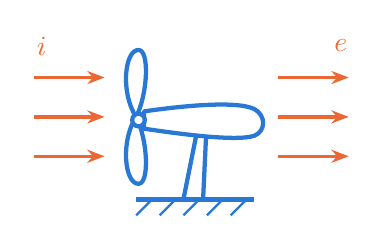
\begin{tikzpicture}[x=1cm, y=1cm,
    flow/.style={-{Stealth[length=2.2mm]}, duRed, line width=1.26pt},
    fan/.style={duBlue, line width=1.54pt, line join=round}]
  % ground and stand
  \draw[fan] (0.95,-1.05) -- (2.45,-1.05);
  \foreach \x in {1.15,1.45,...,2.35}
    \draw[duBlue, line width=0.84pt] (\x,-1.05) -- ++(-0.2,-0.2);
  \draw[fan] (1.55,-1.05) -- (1.72,-0.2);
  \draw[fan] (1.8,-1.05) -- (1.84,-0.2);
  % motor housing
  \draw[fan, fill=white] (1.05,0.07) .. controls (1.4,0.12) and (2.2,0.22) .. (2.45,0.1)
     .. controls (2.6,0.02) and (2.6,-0.18) .. (2.45,-0.24)
     .. controls (2.2,-0.32) and (1.4,-0.2) .. (1.05,-0.15) -- cycle;
  % blades
  \draw[fan, fill=white] (0.95,0) .. controls (0.75,0.3) and (0.8,0.85) .. (0.98,0.85)
     .. controls (1.12,0.85) and (1.1,0.3) .. (0.95,0);
  \draw[fan, fill=white] (0.95,0) .. controls (0.75,-0.3) and (0.8,-0.85) .. (0.98,-0.85)
     .. controls (1.12,-0.85) and (1.1,-0.3) .. (0.95,0);
  \draw[fan, fill=white] (0.98,-0.04) circle (0.08);
  % air in and out
  \foreach \y in {0.5,0,-0.5} {
    \draw[flow] (-0.35,\y) -- (0.55,\y);
    \draw[flow] (2.75,\y) -- (3.65,\y);
  }
  \node[duRed] at (-0.25,0.9) {$i$};
  \node[duRed] at (3.55,0.9) {$e$};
\end{tikzpicture}
\end{document}
